% Created 2020-02-21 Fri 15:00
% Intended LaTeX compiler: pdflatex
\documentclass[11pt]{article}
\usepackage[utf8]{inputenc}
\usepackage[T1]{fontenc}
\usepackage{graphicx}
\usepackage{grffile}
\usepackage{longtable}
\usepackage{wrapfig}
\usepackage{rotating}
\usepackage[normalem]{ulem}
\usepackage{amsmath}
\usepackage{textcomp}
\usepackage{amssymb}
\usepackage{capt-of}
\usepackage{hyperref}
\usepackage[a4paper,margin=1in]{geometry}
\usepackage{fancyhdr}
\pagestyle{fancy}
\lhead{CS1006 P1 GOL \quad{} 190006526 & 190022658}
\rhead{Tutor: Letham \quad{} 21 Feb 2020}
\author{190006526 \& 190022658}
\date{\today}
\title{CS1006 P1 - Game Of Life}
\hypersetup{
 pdfauthor={190006526 \& 190022658},
 pdftitle={CS1006 P1 - Game Of Life},
 pdfkeywords={},
 pdfsubject={},
 pdfcreator={Emacs 28.0.50 (Org mode 9.4)}, 
 pdflang={English}}
\begin{document}

\maketitle
\setlength\parindent{0pt}
\thispagestyle{fancy}

\section{Overview}
\label{sec:orga5cd91c}
In this practical, we were asked to create a GUI program that allowed users to
simulate Conway's Game of Life.  In addition to that, we were asked to add
functionality to load and save \texttt{.gol} files, make the playing field toroidal, and
have alternative rule constants.  We completed that functionality, and
additionally provide the following features in our project:
\begin{itemize}
\item Speed control (using a logarithmic scale)
\item Size control
\item Randomly filling the board
\item Resetting the board
\item Drawing on the board by dragging
\item Toggling between erasing and drawing
\item The ability to enter a custom rule string that changes the rules of the
cellular automata
\item Toggling the colours between displaying the state and the age of a given cell
\item \textbf{3D cellular automata}
\item The ability to save and load 3d files or files with other rule sets
\end{itemize}

The rule string that the user provides is of the following format:
\texttt{<survive>/<born>/<states>/[V/M]}.  The first part, \texttt{survive}, describes the
number of neighbours with which an alive cell survives.  The second part,
\texttt{born}, describes the number of neighbours which a dead cell needs to become an
alive cell.  The third bit, \texttt{states}, describes the number of states in the
cellular automata.  If there are more than two states, states that are neither
alive (always the max state), or dead (the lowest state), decay instead.
These decaying states are not counted as neighbours for alive cells, but can
also not be born while they are still decaying.  For example, in Conway's Game
of Life (Fig 1, Fig 2), there are only two states, dead and alive, or 0 and 1 respectively.
In Brian's Brain (Fig 3), another famous cellular automata, there are three states,
causing the alive cells to leave behind a trail of decaying cells.  The \texttt{[V/M]}
bit describes whether the automata should use the Von Neuman neighbourhood (4
neighbours) or the Moore neighbourhood (8 neighbours), respectively.  Conway's
Game of Life, for example has the rule string: \texttt{2,3/3/2/M}.  A more complex rule
string might look like this: \texttt{2-4/3,4,6-8/24/M} (shown in Fig 4).  Easier to
develop an intuition for what these mean by messing around with the various
samples we have provided.\\

For the colours, the red-yellow gradient represents the state, with red being
the lowest non-dead, and yellow being the highest.  The blue-green gradient
represents the age of the cell, with blue being the oldest, and green the
youngest.  This was implemented to provide additional information about the
cellular automata.\\

For 3D(Fig 5, Fig 6), most of the same rules still apply.  The rule strings don't differ,
except the maximum number of neighbours obviously increases with the extra
dimension.  We were not able to implement a few of the other features, like
colour toggling or drawing/erasing the voxels due to time constraints.  The 3d
part is also prone to freezing if the size/fill percentage is set too high,
because the computer has so much to compute and render.\\

The loading and saving for all of these features is supported.  This was
accomplished by modifying the original file format by adding headers.
Additionally, instead of the \texttt{.} and \texttt{O} characters, we opted to use numbers if the
rule set used more than 2 states.\\

Overall, we are quite proud of what we were able to accomplish on this project.
Below are a few images of what the program is capable of.  We have included
corresponding the files that these images were generated from in the \texttt{saved}
directory of the project.\\

\begin{center}
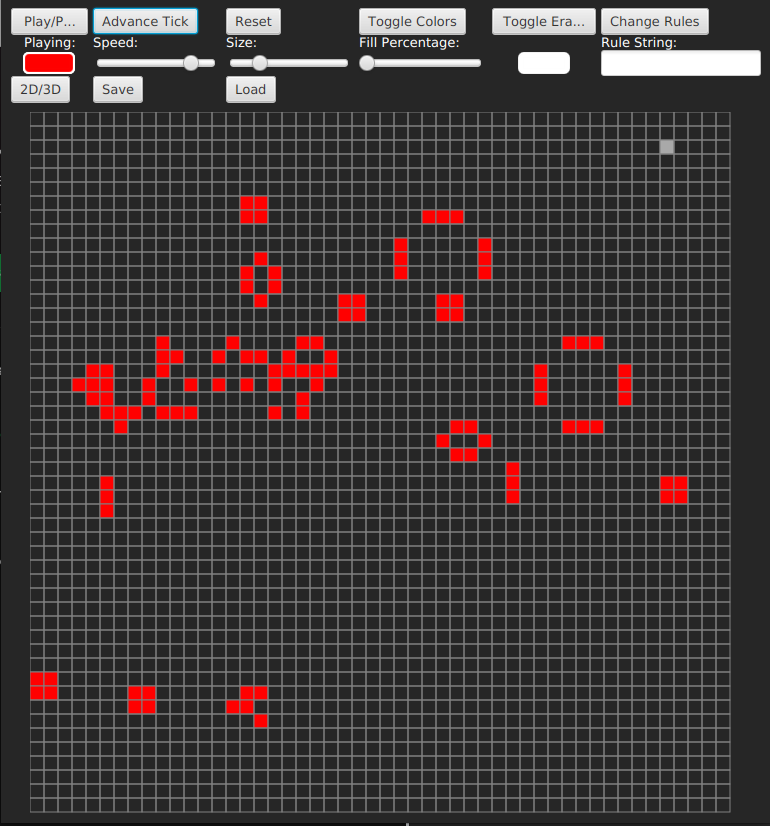
\includegraphics[width=.9\linewidth]{./Fig1.png}
\end{center}
Fig 1.  An ordinary game of life

\begin{center}
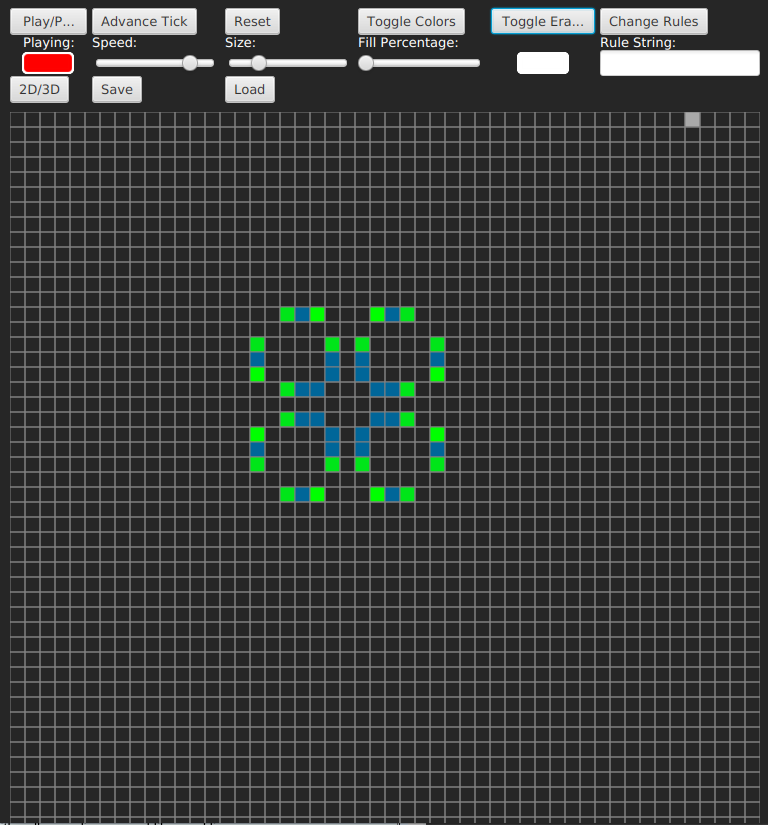
\includegraphics[width=.9\linewidth]{./Fig2.png}
\end{center}
Fig 2:  A pulsar with age colours being shown

\begin{center}
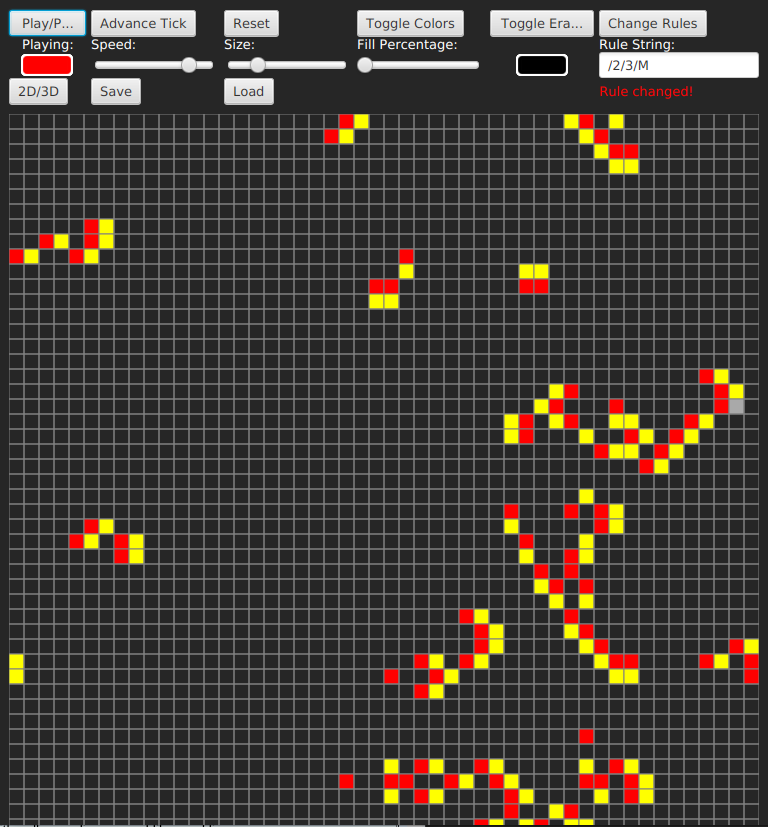
\includegraphics[width=.9\linewidth]{./Fig3.png}
\end{center}
Fig 3: The Brian's brain cellular automaton

\begin{center}
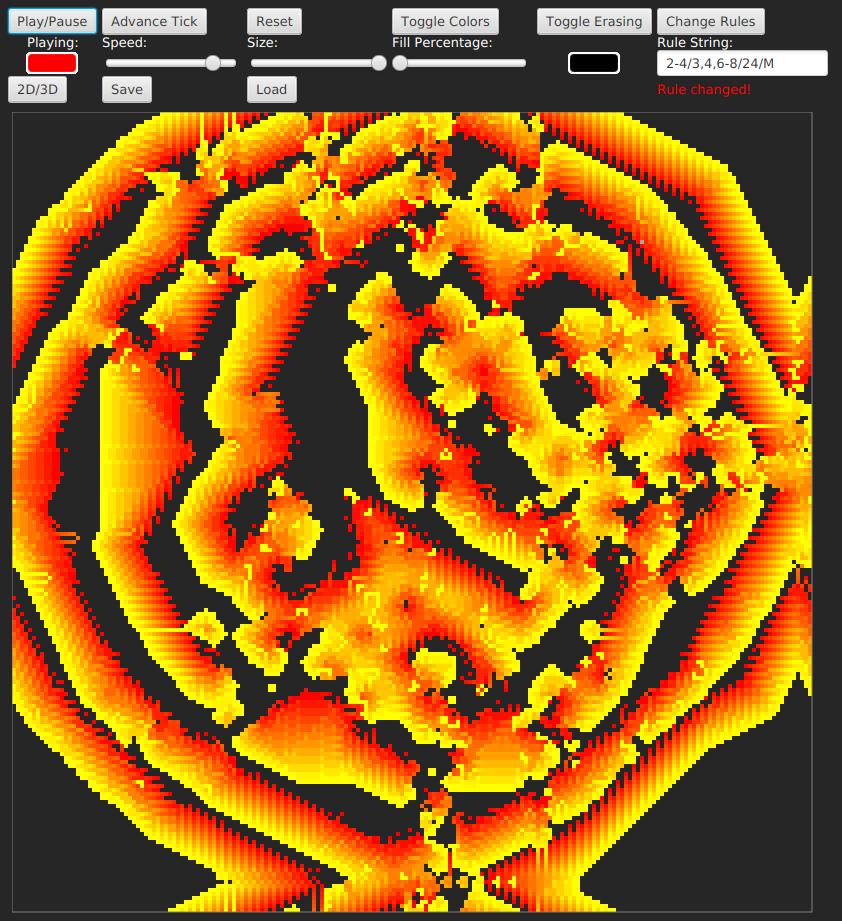
\includegraphics[width=.9\linewidth]{./Fig4.png}
\end{center}
Fig 4:  The ``Bloomerang'' cellular automaton rule

\begin{center}
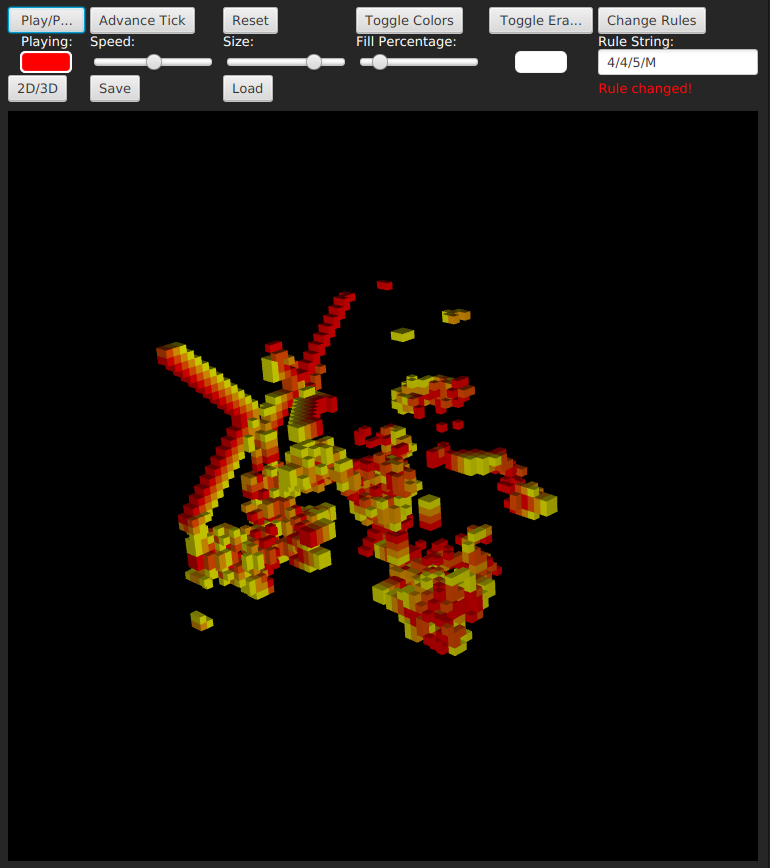
\includegraphics[width=.9\linewidth]{./Fig5.png}
\end{center}
Fig 5: The 445 3d cellular automata
\begin{center}
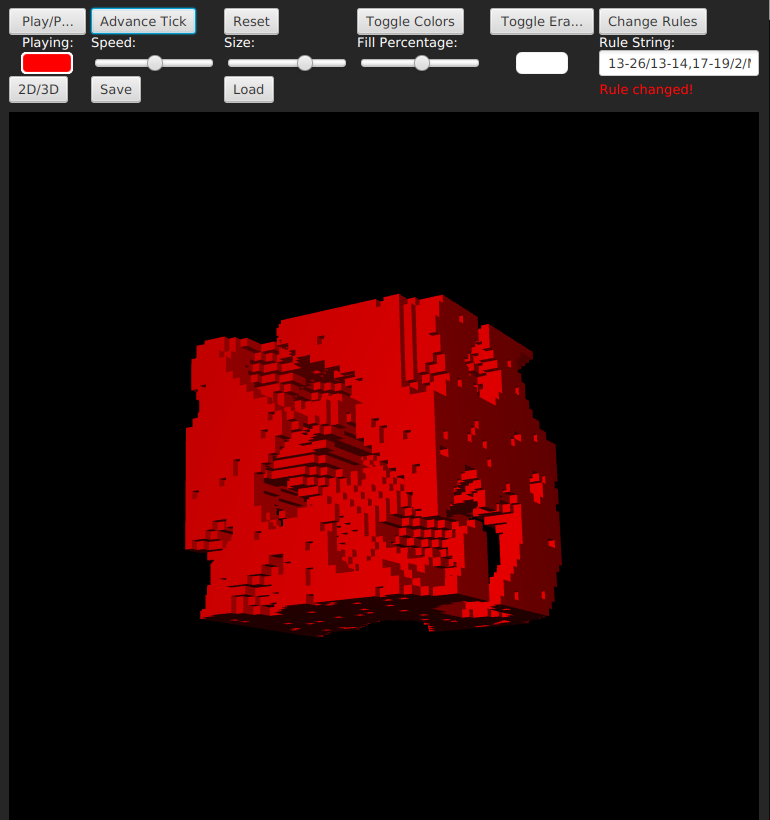
\includegraphics[width=.9\linewidth]{./Fig6.png}
\end{center}
Fig 6: A cave like structure from a 3d cellular automata
\begin{center}
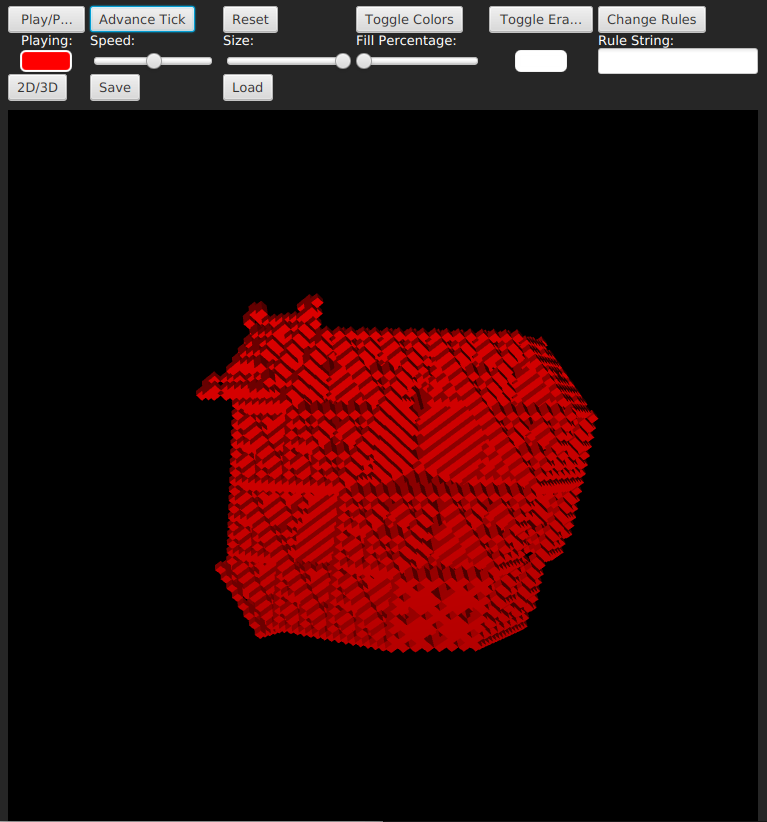
\includegraphics[width=.9\linewidth]{./Fig7.png}
\end{center}
Fig 7: A Sierpinski-like crystal structure forms in this rule set (much easier
to see in the application)
\section{Design}
\label{sec:org37f2b81}
As this project grew in scope, we had to make many decisions on how to structure
the program.  At first, we wrote a very simplistic program using Java's built in
Swing framework, but quickly realised that since we wanted to do 3D as a stretch
goal, we would need something that supported 3D rendering.  Because of this,
JavaFX was something of an obvious choice, as it provides a much more modern
looking interface than Swing, and also provides some bare bones 3D rendering
capabilities.  This was fine, since we didn't need any advanced rendering
features like PBR materials or realtime raytracing.\\

For the structure of logic code, we realized that we would never need more than
one instance of the GameLogic2D, GameLogic3D, and Rule classes at one time, and
passing around each of them would grow messy and confusing.  Because of this, we
opted to use the singleton design pattern, and provide static \texttt{getSingleton()} and
\texttt{setSingleton()} methods for each of these classes.  Although this leads to some
slightly messier lines (GameLogic3D.getSingleton() doesn't exactly roll off the
tongue), in the long run it makes the code much more modular, and it was far
easier to write code knowing that each part of the code would always have the
same valid reference to these instances.\\

For the GUI code, we use the \texttt{MainWindow} class to initialise all of the GUI, and
handle changing between 2D and 3D.  For most of the actions it delegates to the
actual Canvas/Graphics class or the various logic related classes.  The
\texttt{GraphicsRegion} interface provides a common interface (no pun intended) so that the
buttons initialised in \texttt{MainWindow} are able to communicate with the 2D and 3D
graphics the same way.  Listeners are attached to the width and height
properties, and the current \texttt{GraphicsRegion} is told to change its size.  We opted
to use lambda functions instead of anonymous classes for the listeners, because
we never needed to use more than one function, and it cut down on the amount of
clutter in the code.  Although the \texttt{MainWindow} file is fairly long, it isn't
particularly complicated, being mostly composed of setting up the GUI
elements.\\

The \texttt{GameCanvas} class handles the 2D graphics, and uses a custom \texttt{ResizableCanvas}
class that is defined internally to represent the \texttt{Canvas}.   Most of the methods
are fairly self explanatory.  The \texttt{draw} method is the core of the class, and it
runs through all of the different cells on the board, calculating the colour for
each using the appropriate linear gradient.  It then uses the \texttt{fillRect} method to
draw the rectangle the correct colour.\\

The \texttt{Graphics3D} class handles the 3D graphics, and uses JavaFX's built in 3D
capabilities to draw the voxels.  To handle the camera movement, it uses mouse
listeners that rotate the camera.  This functionality was one of the harder
things to figure out, given the notorious complexity of 3D rotations.
Thankfully we didn't have to mess with quaternions or anything crazy.  To draw
the voxels we used the builtin \texttt{Box} class.  For colours we  used the
\texttt{PhongMaterial}, which allows us to use a \texttt{Color} just like we did with the 2D
implementation, without having to mess about with specularity/diffuseness.
Interestingly, the \texttt{GameCanvas} and \texttt{Graphics3D} are fairly comparable in length,
even though the 3D implementation is much more technically complex.  This is
mostly due to the simplicity of JavaFX's 3D API.\\

For the game logic, the code is separated into the \texttt{GameLogic} and \texttt{Rule} classes
(and their subclasses).  Because the \texttt{GameLogic2D} and \texttt{GameLogic3D} have very
little in common due to the 3D version having \texttt{x}, \texttt{y}, and \texttt{z} parameters required
for many of the methods where the 2D version only required the \texttt{x} and \texttt{y}
parameters.  These classes handle all of the logic that happens regardless of
what the current rule is, delegating to the current \texttt{Rule} singleton when needed.
The \texttt{Rule} class and its subclasses handle figuring out whether a given cell lives
or dies, and calculating the number of neighbours a certain cell has.  The
neighbour counting is the only reason the \texttt{Rule} class has the \texttt{Rule2D} and \texttt{Rule3D}
subclasses.  Importantly, \texttt{Rule} also contains the static \texttt{parseRuleString(String,
boolean)} method, which validates a rule string and then returns a new \texttt{Rule} that
conforms to the String.\\

For file IO, the aptly named \texttt{IO} class is used.  It uses JavaFX's \texttt{FileChooser}
class, because it provides a very nice ready-made file browser to save and load
files with.  This way we don't have to spend much time validating filepaths
ourselves, and can instead focus on getting the file format right.  Our version
starts with a 3 line header.  This header includes the rule string, the size,
and whether it is 3D, in that order.  After that it stores the data in plain
text, either as \texttt{.} and \texttt{O} for 2 state cellular automata, and uses integers
separated by spaces for anything else.  This is certainly not the most efficient
file format, but it is a fairly easy one to read, and it is easy to hand modify
it because it's in plaintext.  Having to manually edit it in a hex editor would
be less than ideal.  For 3D files, the same format is used, with each layer
placed after the last, with no delimiter between.

That is most of the architecture covered.  The code is for the most part fairly
well structured, but in the IO class we ended up writing a bit of hacky code to
update the \texttt{GraphicsRegion} to the correct version (3D/2D).
\section{Bugs}
\label{sec:orgfdb8c37}
The primary bug we have currently is in the 3D section of the program.  In this
section, if there are two many cubes on the screen, the program will slow to a
crawl and then freeze up, requiring a restart.  This bug is caused by lack of
optimisation to the rendering process, which would quite frankly require us to
use something other than JavaFX's builtin 3D graphics.  While this is not an
impossible feat, it is so vastly outside the scope of the project that we
decided not to pursue it.  Many of the high quality videos of 3D cellular
automata found online are done using rendering software like Blender over many
hours to produce a 30 second clip of video, so it is not reasonable for our
program, especially given the limitations of JavaFX, to do this in real time.
Perhaps one day we can return to this and try to fix it.  Because of this issue,
users of the program should use normally use the ``advance tick'' button instead
of the play/pause button when using the 3D section.\\

As well as this bug, there is a bug we haven't figured out how to reproduce
where there is an out of bounds exception upon opening the file.  Since this is
so sporadic, it may be caused by something like a race condition, but we haven't
been able to track it down.  Luckily, it doesn't crash the program, it just
throws an exception.

\section{Build Instructions}
\label{sec:orge71745a}
Because the gradle wrapper install gradle locally and also installs the
dependencies (JavaFX),  you shouldn't need to install anything yourself.
\subsection{Linux/Mac}
\label{sec:org904215a}
\begin{enumerate}
\item Clone the repository ( \texttt{hg clone https://of9.hg.cs.st-andrews.ac.uk/GameOfLife} )
\item Run \texttt{./gradlew run} from the top level of the directory
\end{enumerate}
\subsection{Windows}
\label{sec:orgdfa1136}
\begin{enumerate}
\item Clone the repository ( \texttt{https://of9.hg.cs.st-andrews.ac.uk/GameOfLife} )
\item Run \texttt{.\textbackslash{}gradlew.bat run} from the top level of the directory in
PowerShell
\end{enumerate}
\section{Usage Instructions}
\label{sec:org3b5e150}
Most of the program has already been described, but there are a few things to
note about using it.  Because of the slowness experienced when using the 3D
mode, it is best to use the advance tick in the beginning, until the amount of
voxels has thinned out.  In the case of Fig6.gol and Fig7.gol, the play/pause
button should not be used, as it will slow and then freeze the program.  With
Fig5.gol it should be fine to use the play button.\\

For some interesting cellular automata to try, check the following:
\begin{itemize}
\item \url{http://psoup.math.wisc.edu/mcell/rullex\_gene.html}
\item \url{https://softologyblog.wordpress.com/2019/12/28/3d-cellular-automata-3/}
\end{itemize}

\textbf{Word Count: 2019}
\end{document}
